\section{El proceso de desarrollo de videojuegos}
\subsection{Introducción}
El desarrollo de un videojuego, como el de cualquier otro producto software, debe de ser planificado correctamente y ejecutado siguiendo una metodología adecuada. Sin embargo, El diseño y desarrollo de un videojuego requiere de la participación de campos ajenos a la informática como el diseño de juegos, el diseño gráfico o la composición musical. Una parte importante de la producción consistirá en organizar a un equipo multidisciplinario para poder terminar el proyecto dentro del tiempo y presupuesto acordados \cite{libro_esi}.

\begin{figure}[h]
    \centering
    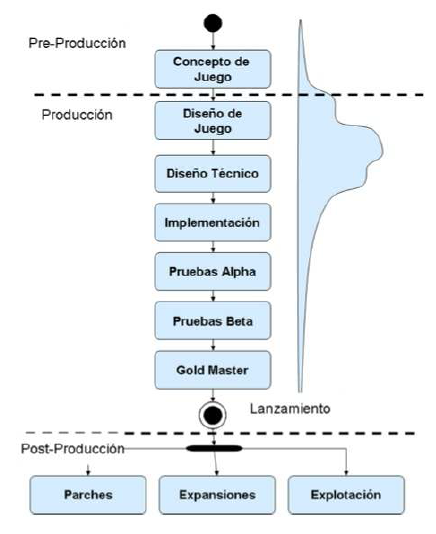
\includegraphics[width=0.6\textwidth]{images/estadodelarte/desarrollo/etapas-desarrollo}
    \caption{Tabla extraída del libro ``Curso de Experto en Desarrollo de Videojuegos''.}
\end{figure}

\subsection{Etapas del desarrollo}
\subsubsection{Desarrollo del Concepto}
El desarrollo de todo videojuego comienza con una idea. Durante la fase de desarrollo del concepto se tomará dicha idea para obtener un diseño preliminar listo para pre-producción. El objetivo principal de esta etapa es decidir sobre qué tratará el juego y ponerlo por escrito para que cualquier miembro del equipo lo pueda entender con claridad, decidiendo las principales mecánicas, creando el arte conceptual y escribiendo el argumento\cite{game_design_2}. 

Al final de la etapa se habrán elaborado tres documentos: El \textit{High Concept}, el \textit{Pitch Document} y el \textit{Concept Document}. El High Concept consiste en una o dos frases que describen a grandes rasgos cómo será el juego, en especial que lo hace distinto de la competencia. El \textit{Pitch Document}, o Propuesta de Juego, es un pequeño documento de en torno a dos páginas, orientado a ser leído en las reuniones donde el juego sea propuesto a inversores. El documento resume las características del juego y explica por qué será exitoso y rentable.

Finalmente, el \textit{Concept Document} es un extenso documento que explica en detalle las características del juego. Se trata de una versión extendida de \textit{Pitch Document} que trata temas como: 
\begin{itemize}
\item El High Concept
\item El género del juego
\item Características principales y jugabilidad.
\item Ambientación e historia.
\item Estimación del presupuesto y de la planificación.
\item Equipo de desarrollo.
\item Análisis de Riesgos.
\end{itemize}

\subsubsection{Pre-Producción}
La pre-producción es la fase de preparación: en la que el equipo diseña y planifica los elementos que serán desarrollados en la etapa de producción. Al final de esta etapa, se debe haber completado el diseño de juego, creado la biblia de arte, elaborado el documento de diseño técnico, establecido el plan de producción, y creado un prototipo del juego final\cite{game_design_2}.

El diseño del juego quedará establecido en un Documento de Diseño de Juego (o GDD, por sus siglas en ingles). Se trata de un documento ``vivo'', que está en constante modificación para adaptarse a los ajustes concretos de diseño que se realizarán durante el desarrollo.

La biblia de arte es una colección de arte conceptual que servirá para definir el estilo artístico del juego desde un primer momento. La biblia incluirá también una librería de imágenes de referencia que puedan ser de ayuda a los artistas que desarrollen los elementos gráficos finales.

El Documento de Diseño Técnico contiene una descripción en detalle la parte técnica del proyecto definiendo las tareas que los desarrolladores deberán afrontar, estimando el coste que dichas tareas tendrán tanto en tiempo como en número de personas y especificando las herramientas y técnicas que utilizará el equipo.

El Plan de producción recopila la información acerca de cómo se va a desarrollar el proyecto. Este incluye las tareas a realizar junto a los tiempos, costes y dependencias de estas, divididos en varios documentos menores para poder ser organizado mejor:
\begin{itemize}
\item \textbf{Plan de mano de obra}: Listado del personal, sus horarios y su salario.
\item \textbf{Plan de recursos} Estimación del coste los recursos externos al proyecto (música, arte, herramientas...)
\item \textbf{Documento de seguimiento}: Documento donde se realiza un control de los tiempos y plazos del proyecto.
\item \textbf{Presupuesto}: Contiene el coste mensual del proyecto y el cálculo del presupuesto general
\item \textbf{Ganancias y Pérdidas}: Estimación  de las ganancias y  pérdidas del proyecto. Debe ir actualizándose según se avanza en el desarrollo.
\item \textbf{Definición de Hitos}: Lista de las distintas "metas" del proyecto, que son puntos del desarrollo donde se habrá terminado una cantidad de trabajo importante.
\end{itemize}

Una vez diseñado y planificado el proyecto, el equipo empezara a trabajar en la creación de un Prototipo. Un prototipo es una pieza de Software funcional que contiene una pequeña fracción del software final. El desarrollo prototipo servirá para varias funciones: poner a prueba el diseño de juego, concretando de forma más precisa la jugabilidad; realizar un simulacro de desarrollo para determinar las dinámicas del equipo y producir una muestra del juego final a inversores y publicadores.

\subsubsection{Producción}
La producción es la etapa principal del desarrollo del juego. Durante esta etapa se elaborarán e implementarán los elementos descritos y diseñados durante la pre-producción: los programadores implementarán los sistemas del juego, los artistas elaboraran los gráficos definitivos, los diseñadores crearán misiones y niveles, etcétera. Dependiendo del juego en cuestión, una producción normal suele durar entre seis meses y dos años, aunque el desarrollo de juegos pequeños para, por ejemplo, dispositivos móviles puede realizarse en menos tiempo aún.

La etapa de producción es de naturaleza iterativa: El juego va construyéndose en varias etapas en las que se implementan pequeñas porciones de este. Entre etapa y etapa, el juego pasa por un proceso de pruebas en la que se verifica su usabilidad y robustez frente a fallos. Los resultados de las etapas se utilizan como base para recalcular los tiempos y presupuestos de las etapas posteriores. Dividir el desarrollo de esta forma hace que sea más sencillo afrontar problemas y contratiempos que el equipo podría encontrar en las etapas tardías.

\subsubsection{Final de Producción y Lanzamiento}
Durante las últimas etapas de la producción, el paradigma de desarrollo cambia, pasando el objetivo de implementar contenido nuevo a pulir y ajustar el contenido preexistente. Esta parte de la producción puede dividirse en dos etapas: Alpha y Beta.

La fase \textbf{Alpha} o Code-Complete es el punto del desarrollo donde el juego se encuentra en un estado jugable, a falta solo de ciertos vacíos como gráficos provisionales o mini juegos o sub-sistemas incompletos. El objetivo de esta etapa es el de encontrar y corregir todos los fallos posibles y también probar y ajustar la jugabilidad\cite{development_and_production}.

En la fase \textbf{Beta} o Content-Complete la mayor parte del contenido del juego deberá estar terminado y debe haber pocos o ningún fallo importante en el juego. En esta etapa el juego es puesto en manos de equipos de testing externos a la empresa para realizar análisis exhaustivos en busca de fallos que se le pueden haber escapado al equipo de testing interno. Es también en esta etapa donde la campaña de publicidad del juego deberá ser más fuerte\cite{development_and_production}.

Una vez superadas las dos etapas de pruebas, la Versión Final del juego es enviada a la distribuidora para que comience la producción de las copias físicas, o para que el juego aparezca en las plataformas de distribución.

\subsubsection{Post-Producción}
Una vez lanzado el juego, el equipo entra en la etapa de Post-Producción. En esta etapa el equipo trabajará en corregir fallos y problemas que los jugadores encontraron tras el lanzamiento y en la elaboración de contenido adicional descargable.

La duración y trabajo de la post-producción depende mucho del juego en cuestión. Hasta hace relativamente poco, los juegos lanzados en videoconsolas carecían completamente de esta etapa debido a la dificultad para modificar los juegos que ya se encontrasen en el mercado. por otro lado, hoy en día la mayor parte de los videojuegos reciben parches y actualizaciones sin importar su plataforma de distribución\cite{development_and_production}.

Un caso especial sería el de los juegos con un fuerte componente Online, como los MMORPG, los MOBA o los shooter en línea. Los desarrolladores de este tipo de juegos, para mantener contenta a su base de jugadores y evitar el estancamiento, lanzan de forma periódica actualizaciones que ofrecen nuevo contenido, mejoras y ajustes. Algunos de estos juegos pueden recibir este tipo de actualizaciones durante años, como World of Warcraft\footnote{https://worldofwarcraft.com (MMORPG de Blizzard, en activo desde 2004)} o Team Fortress 2\footnote{teamfortress.com/} (FPS de Valve, en activo desde 1999)

\subsection{Estructura típica de un equipo de desarrollo}
El desarrollo de un videojuego puede llevarse a cabo por equipos de desarrollo muy distinto dependiendo de la extensión del proyecto, desde una sola persona creando un pequeño juego independiente, el cual realiza todo el trabajo por sí mismo; hasta los equipos de cientos de personas que desarrollan los juegos "triple A", organizados en múltiples departamentos, cada uno con su estructura jerárquica.

A pesar de esto, existen una serie de roles que están presentes en todos los desarrollos. En los proyectos pequeños será normal encontrar que una misma persona ejerce varios roles, mientras que las grandes compañías pueden tener departamentos enteros encargándose de un único rol.

\begin{figure}[h]
    \centering
    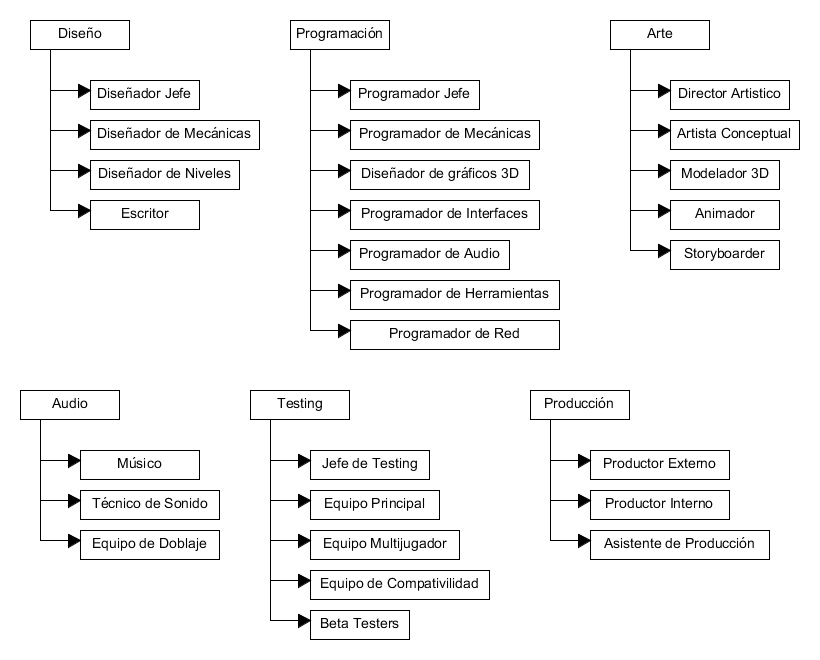
\includegraphics[width=0.8\textwidth]{images/estadodelarte/desarrollo/table-roles}
    \caption{Distribución de roles en un equipo de desarrollo.}
\end{figure}

\subsubsection{Diseño}
La primera y más importante parte del desarrollo de un juego es el Diseño de este. El trabajo del diseñador es de describir el juego con un alto nivel de detalle, definiendo de con precisión todas las mecánicas, personajes, mapas, misiones del juego. Deberá también, hasta cierto punto, coordinar y dirigir el trabajo del resto de miembros del equipo para que puedan implementar correctamente el juego. 

En equipos grandes, el rol de diseñador puede dividirse en las siguientes categorías\cite{development_and_production}:
\begin{enumerate}
\item \textbf{Diseñador Jefe}: Es el encargado de dirigir al resto de diseñadores, decidiendo que contenido entra o no en el juego. Suele ser la persona que tuvo la ``idea'' original del juego.
\item \textbf{Diseñador de mecánicas}: El diseñador de mecánicas es el encargado de diseñar los distintos sistemas de juego, sirviendo como puente entre el diseñador jefe y los programadores. Debido a esto, el diseñador de mecánicas suele tener un trasfondo de programador.
\item \textbf{Diseñador de niveles}: También llamados diseñadores de misiones, son los encargados de crear las distintas etapas que componen el juego, ya sean niveles, misiones, desafíos o puzles.
\item \textbf{Escritor}: La tarea del escritor es la de crear la historia del juego, así como la de escribir los distintos textos de este, como diálogos o descripciones. Se trata de una tarea muy distinta de la de un escritor de novelas o de guiones de película, ya que debe conciliar la narrativa con las exigencias de otros componentes del juego como el diseño, el arte o las limitaciones técnicas.
\end{enumerate}
\begin{figure}[h]
    \centering
    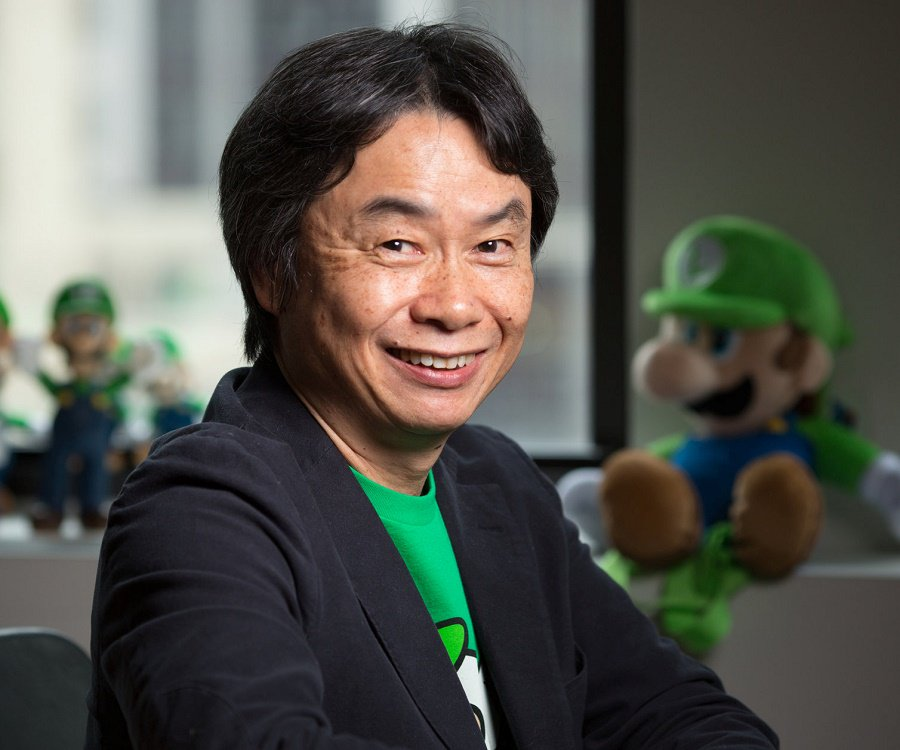
\includegraphics[width=0.45\textwidth]{images/estadodelarte/desarrollo/shigeru-miyamoto}
    \caption{Shigeru Miyamoto (creador de Super Mario, Zelda y Donkey Kong) es posiblemente el diseñador de videjouegos más famoso}
\end{figure}

\subsubsection{Programación}
El rol del programador es el de implementar el juego en forma de código ejecutable. Esto supone el diseño e implementación de todo tipo de componentes imprescindibles: motor de renderizado, librerías para trabajar con sistemas de audio o conectarse por Internet, herramientas para integrar fácilmente el contenido artístico entre otras.

Cuando el equipo de desarrollo es grande, el rol de programador tiende a dividirse para cubrir tareas más específicas\cite{development_and_production}:
\begin{enumerate}
\item \textbf{Programador Jefe}: El programador jefe es frecuentemente el programador con más experiencia del equipo y él es el encargado de resolver las tareas más complicadas e importantes del proyecto. Cuando el equipo es muy grande, suelen realizar también tareas de coordinación.
\item \textbf{Programador de Mecánicas}: Es el encargado de convertir el diseño de juego en código ejecutable. Entre sus tareas se encuentra definir las físicas del mundo del juego, definir las funciones de los distintos objetos y modelar el comportamiento de los personajes.
\item \textbf{Programador de gráficos 3D}: Es el responsable de implementar los sistemas para la creación y renderizado de gráficos 3D. El programador de gráficos 3D necesita contar con conocimientos avanzados en calculo, matemática vectorial y matricial, trigonometría y álgebra.
\item \textbf{Programador de Interfaces}: Es el encargado de implementar los sistemas de interacción entre el jugador y el juego, normalmente interfaces de control, menús y HUDs (Head-Up Displays). 
\item \textbf{Programador de Audio}: Es la persona responsable de la implementación de los distintos sistemas que se utilizarán para reproducir música y sonido en el juego
\item \textbf{Programador de Herramientas}: El programador de herramientas tiene la responsabilidad de crear las distintas herramientas que el resto del equipo pueda necesitar para realizar, o acelerar, su trabajo. Un tipo especializado de programador de herramientas es el programador del editor de niveles, debido a la importancia de esta herramienta para el desarrollo del juego y por la posibilidad de que dicho editor sea lanzado al público como parte del juego.
\item \textbf{Programador de Red}: Es el encargado de escribir el código que permite a los juegos ser ejecutados entre varios equipos, ya sea código máquina de bajo nivel o la integración de un librería de alto nivel.
\end{enumerate}
\begin{figure}[h]
    \centering
    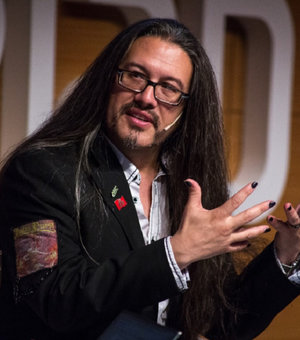
\includegraphics[width=0.35\textwidth]{images/estadodelarte/desarrollo/john-romero}
    \caption{Jonh Romero es el co-fundador de ID Software y programador de juegos como Doom o Quake}
\end{figure}

\subsubsection{Arte}
Se denomina artista a la persona o grupo encargado de generar los componentes gráficos del juego: modelos 3D de personajes y objetos, texturas, diseño de menús e interfaces, bocetos, animaciones y demás.

Existen varias categorías de artistas distintas dependiendo de en qué rama se especialicen y de cuál sea su rol en la estructura del proyecto\cite{development_and_production}:
\begin{itemize}
\item \textbf{Director Artístico}: Asignado al artista con mayor experiencia en la industria, el papel del director artístico es el de organizar y coordinar al resto de artistas para que realicen correctamente su trabajo y el de revisar las piezas producidas para asegurarse de que son consistentes con el estilo artístico establecido.
\item \textbf{Artista Conceptual}: El artista conceptual es el encargado de producir bocetos provisionales que servirán como base para construir los gráficos definitivos del juego.
\item \textbf{Artista 2D}: Los artistas 2D son expertos en las técnicas tradicionales del dibujo y pintura.  Su rol es más notable en los juegos 2D, donde deben producir la mayoría de los componentes gráficos como fondos, \textit{tiles} y \textit{sprites}; pero también tienen un papel notable en los juegos 3D, donde suelen ser los encargados de diseñar interfaces gráficas, crear las texturas de los modelos 3D e incluso realizar trabajos ajenos al propio juego como la creación de imágenes promocionarles.
\item \textbf{Modelador 3D}: Es el encargado de producir los modelos 3D de los distintos componentes del juego tales como personajes, objetos, mapas...  Es relativamente común que los modeladores 3D tengan ciertos conocimientos de programación debido a que eran necesarios para trabajar con los primeros programas de modelado 3d.
\item \textbf{Animador}: Es el encargado de animar los diferentes elementos del juego, desde el simple movimiento de un molino de viento hasta las complicadas expresiones de una cara. Existen dos alternativas para realizar la animación: la técnica de keyframing, que consiste en realizar poses estáticas de los personajes que el programa utiliza para generar la animación; y la captura de movimiento, en la que los movimientos de un actor son capturados y transferidos al juego mediante un equipo especializado.
\item \textbf{Storyboarder}: Es el artista encargado de diseñar escenas del juego. Para ello, el Storyboarder crea unas secuencias de arte conceptual que describen los tiempos, diálogos y eventos de las escenas, lo que permite valorarla y validarla antes de iniciar el costoso proceso de producción.
\end{itemize}
\begin{figure}[h]
    \centering
    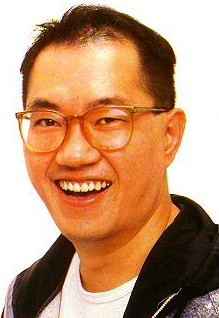
\includegraphics[width=0.25\textwidth]{images/estadodelarte/desarrollo/akira-toriyama}
    \caption{Akira Toriyama, el autor de Dragon Ball, ha trabajado como artista en juegos como Dragon Quest o Chrono Trigger}
\end{figure}

\subsubsection{Audio}
El trabajo de audio en un videojuego viene en tres categorías: música, efectos de sonido y doblaje. Existen especialistas que se dedican exclusivamente a una sola de estas categorías, aunque no es raro encontrarse en pequeños estudios a una persona encargarse tanto de la música como del sonido. Reflejando los tipos de audio, los tres tipos de profesionales son\cite{development_and_production}:
\begin{enumerate}
\item \textbf{Músico}: Es el artista encargado de escribir las composiciones musicales que se escucharán a lo largo del juego. Es muy común que el músico también se haga cargo de interpretar sus composiciones mediante programas de síntesis de música, aunque las grandes producciones pueden permitirse contratar interpretaciones en vivo.
\item \textbf{Técnico de sonido}: Los técnicos de sonido son profesionales que se dedican a fabricar o adaptar sonidos para el proyecto en el que trabajen.
\item \textbf{Equipo de doblaje}: El trabajo de doblar un videojuego requiere del trabajo de varios profesionales. En primer lugar, está el actor de voz, un actor especializado que interpreta con su voz a uno o varios personajes del juego. El trabajo de los actores está supervisado por un director de doblaje, que además suele encargarse de adaptar el guion y de dirigir a los técnicos de sonido que van a grabar y manipular las voces.
\end{enumerate}
\begin{figure}[h]
    \centering
    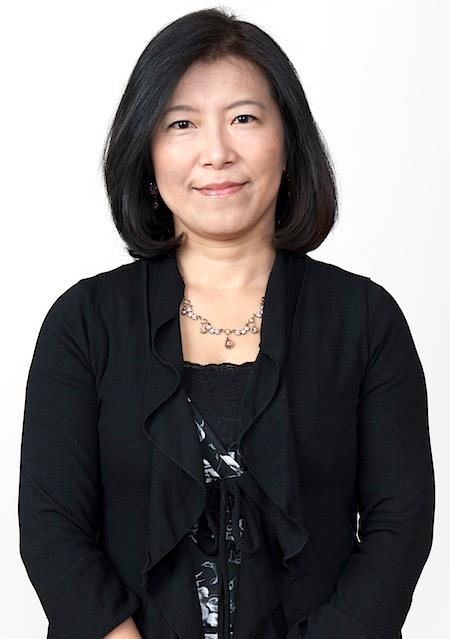
\includegraphics[width=0.25\textwidth]{images/estadodelarte/desarrollo/yoko-shimomura}
    \caption{Yoko Shinomura es una compositora conocida por su trabajo en videojuegos como Final Fantasy o Street Fighters}
\end{figure}

\subsubsection{Testing}
El Aseguramiento de la Calidad (o QA por sus siglas en inglés) es un requisito clave para el desarrollo de un videojuego, a la vez de un proceso lento y costoso que debe comenzarse lo más pronto posible para evitar un sobrecoste\cite{development_and_production}. El trabajo del tester es el de revisar las distintas versiones del juego en busca de fallos para que los desarrolladores puedan arreglarlos.

Normalmente, los testers de un juego se agrupan en equipos, dirigidos por un jefe de testing. Cada equipo de testers se encarga de revisar una faceta distinta del juego, el equipo principal se encarga de probar la jugabilidad y los modos de juego individuales, el equipo multijugador se ocupa de revisar la jugabilidad en línea, así como los componentes técnicos de las conexiones, el equipo de compatibilidad prueba el juego en diversas plataformas y PCs con distintos componentes y el equipo de localización comprueba que se halla realizado una correcta traducción a distintos idiomas.

Para evitar la pérdida de punto de vista critico que el equipo principal y el equipo de multijugador pueden sufrir tras haber trabajado con el juego desde el principio del desarrollo, es normal cambiar los equipos en las últimas etapas del desarrollo por equipos nuevos que no estén involucrados en el juego.

Junto al trabajo de los equipos profesionales de testing se suelen realizar campañas de Beta Testing. El Beta testing consiste en liberar una versión incompleta del juego para que jugadores aficionados los prueben. Las resultados y opiniones de los jugadores son recogidos para utilizarse en el desarrollo de la versión completa. Para realizar una exitosa campaña de beta testing es necesario contar con uno o más organizadores que puedan gestionar la retroalimentación de los usuarios.

\subsubsection{Producción}
La función principal del productor es servir de puente entre el equipo de desarrollo y el resto de la empresa. El productor debe tener un conocimiento profundo del juego y de los demás miembros del equipo, de forma que pueda explicarlo de forma correcta en las mochas reuniones que se tendrán con otros departamentos, como por ejemplo el de marketing\cite{game_design_2}.

El productor se encarga de realizar la gestión del proyecto, coordinando al equipo, realizando la programación de las etapas del proyecto y gestionando los posibles riesgos.

Existen tres tipos de productores dependiendo de su especialidad. Estos son:
\begin{enumerate}
\item \textbf{Productor Externo}: Este tipo de productor trabaja para la compañía editora y se encarga de supervisar al equipo de desarrollo para asegurarse de que se cumplen los acuerdos establecidos por ambas partes.
\item \textbf{Productor Interno}: Esta clase de productor trabaja en la compañía desarrolladora y se encarga tanto de realizar una gestión interna del proyecto como de actuar de representante de del equipo.
\item \textbf{Asistente de Producción}: Los asistentes de producción se encargan de realizar las tareas a las que el productor jefe del proyecto no puede dedicarse personalmente. Normalmente se trata administrar detalles concretos como administrar recursos, realizar el papeleo o gestionar los servidores y la página web.
\end{enumerate}
